\documentclass{article}


% load package with some of the available options - you may not need this!
\usepackage[framed,autolinebreaks,useliterate]{mcode}

% for checklist
\usepackage{enumitem,amssymb}
\newlist{todolist}{itemize}{2}
\setlist[todolist]{label=$\square$}
\usepackage{pifont}
\newcommand{\cmark}{\ding{51}}%
\newcommand{\xmark}{\ding{55}}%
\newcommand{\done}{\rlap{$\square$}{\raisebox{2pt}{\large\hspace{1pt}\cmark}}%
\hspace{-2.5pt}}
\newcommand{\wontfix}{\rlap{$\square$}{\large\hspace{1pt}\xmark}}


% something NOT relevant to the usage of the package.
\usepackage{graphicx}
\usepackage{float}
\usepackage{url,textcomp}
\setlength{\parindent}{0pt}
\setlength{\parskip}{18pt}
\title{ECTA Homework 3\\Shape Matching Problem}
\author{Debaraj Barua (9030412), Md Zahiduzzaman (9030432)}
% //////////////////////////////////////////////////

\begin{document}

\maketitle
\begin{center}
	\begin{minipage}{1\linewidth}
		\centering
			
\includegraphics[scale=0.6]{img/wingtypes.png}
	\end{minipage}
\end{center}

To optimize wings, it is useful to start with known designs and then adjust them to specific tasks. How to convert from one representation to another? In this assignment you will convert the 4-dimensional NACA wing specific representation into a general B-Spline representation with 32 control points. You will compare 2 evolutionary methods, Genetic Algorithms and Evolution Strategies.

\newpage

\section{Assignment Description}
	Shape Matching Problem
	\begin{enumerate}
		\item Write your own Genetic Algorithm to solve the shape matching problem
		\item Write your own version of the Covariance Matrix Adaptation Evolution Strategy (CMA-ES) to solve the shape problem.
		\item Compare the performance of the two algorithms on three airfoils (NACA airfoil shapes: 0012, 5522, 9735). Is there a significant difference between a GA and an ES? 
	\end{enumerate}

	\begin{itemize}
 	\item Grading Scheme
 		\begin{todolist}
 		\item Genetic Algorithm (20 pts)
 			\begin{todolist}
 			\item Bitstring \textit{or }Real-Valued ($20$ pts)
 			\item Bitstring \textit{and }Real-Valued ($+10$pts)
 			\end{todolist}
 		\item Evolution Strategies (60 pts)
 		  	\begin{todolist}
 			\item ES with $1/5$ rule ($30$ pts)
 			\item CMA-ES with out evolution paths ($30$ pts)
 			\item CMA-ES with evolution paths ($+10$)
 			\end{todolist}
 		\item Comparisons (20 pts)
 		  	\begin{todolist}
 			\item Big beautiful wall of data
 			\end{todolist}
 		\end{todolist}
	\end{itemize}
\newpage


\section{Submission Instructions}
To be perfectly clear we expect two submissions to LEA:
\begin{enumerate}
	\item 1 PDF (report) -- a modified version of your submission PDF, with your own code snippets, figures, and responses inserted
	\item 1 ZIP (code and data)   -- a .zip file containing all code use to run experiments (.m files) \textit{and} resulting data as a .mat file
	\item Make sure to follow the naming scheme\newline HW\_NUMBER\_LASTNAME1\_LASTNAME2.suffix
	\item $\rightarrow$ A valid name would be HW\_02\_Smith\_Fernandez.pdf
	\item Make sure both team members use the same filename!
\end{enumerate}

\newpage


\newpage
\section{The Assignment}

\subsection{Genetic Algorithm}
\begin{itemize}
	\item Genetic Algorithms are typically represented by a string, this string could take many forms, such as bitsrings or real-valued numbers. What are the advantages and disadvantages of each encoding in this application? How would you convert each into 32 real-valued numbers? How could you perform crossover and mutation in each? Which do you think would be best?
	\begin{enumerate}
		\item Bitstring
		\\\color{blue}
		One way to represent the problem will be to represent each estimate for the Y value as the binary representation of the number. 
		
		The advantage of such an approach will be ease of mutation of the bit string by bit flips. On creating new individuals in this manner, we would however have to ensure each individual lies within the given range. Another advantage would be that we can avoid round off errors resulting from floating point operations using real valued numbers.
		
		Crossover can be implemented as a single point crossover, where we create new individual from the two parts of each parent.
		
		Mutation can be implemented by a bitflip according to a mutation probability.
		
		\color{black}
		\item Real-valued
		\\\color{blue}
		\textbf{Representation}:
		A string of 32 real valued numbers between -0.5 to 0.5 can be used to represent the problem. These 32 numbers together are a representation of a single genome with possible values of the estimates of Y-value against the control points.
		
		\textbf{Advantage}: These values can be used to represent the Y position of the 32 control points directly, this makes it easy to check the fitness by comparing with the actual value.
		
		\textbf{Disadvantage}: Round off error in floating point operations.
		
		 
		\textbf{Crossover}: Crossover is achieved by taking two parent ids and then getting the mean of the their genomes depending on the crossover probability. This mean value is used to represent a new child genome.  
		
		\textbf{Mutation}: It is achieved by generating gene values between -0.5 and 0.5 to replace genes based on the mutation probability.
		
		
		\color{black}
	\end{enumerate}
	\item Implement the encoding you think will perform best and plots its median performance over 20 iterations, using 20,000 evaluations.
	\\\color{red}Your plot here\color{black}
			\begin{figure}[H]
				\centering
				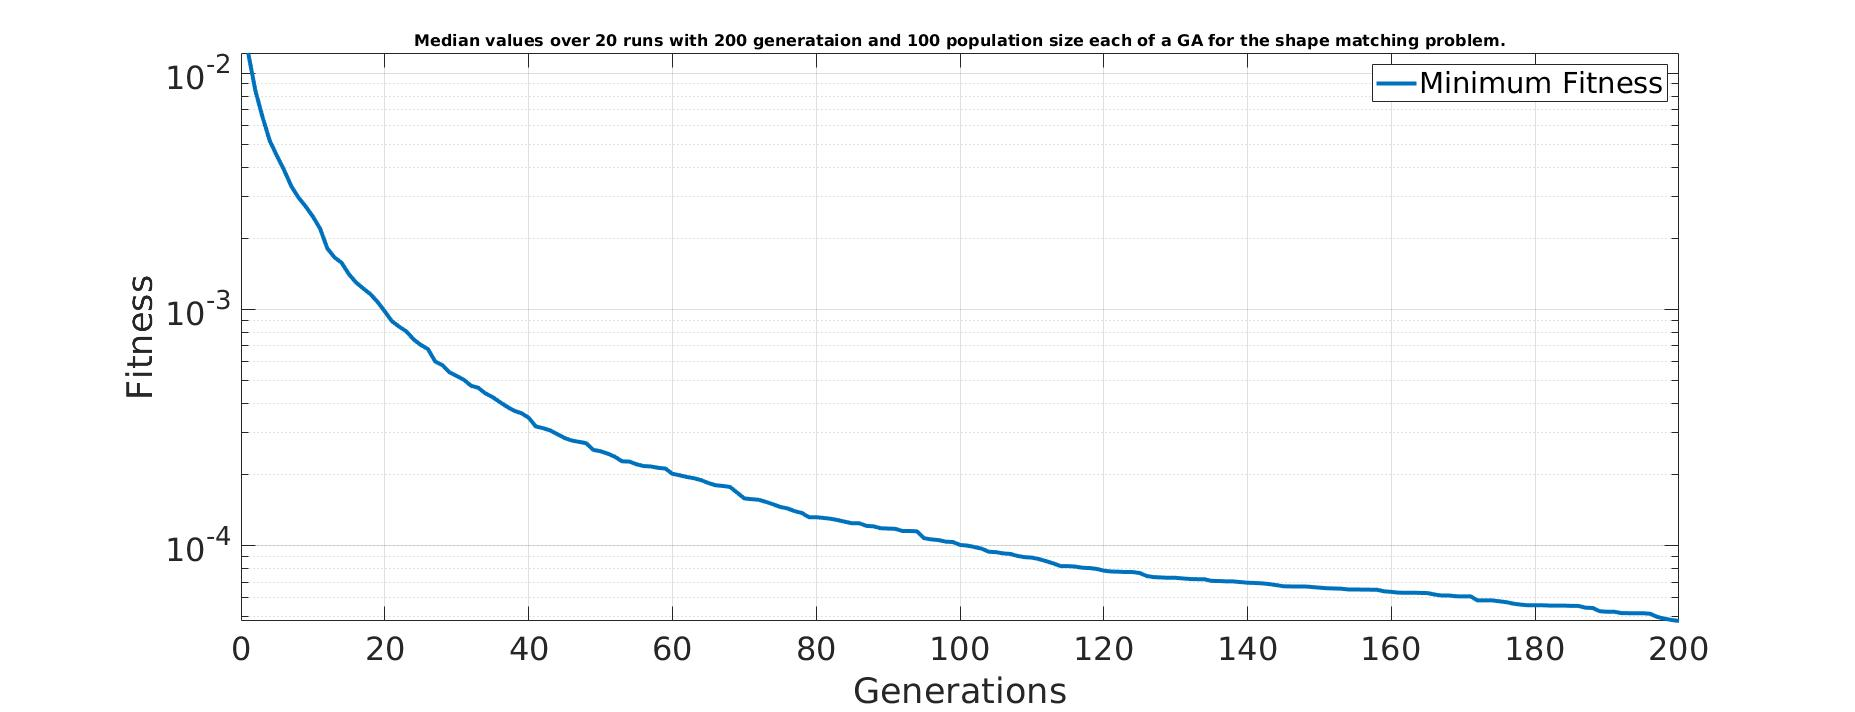
\includegraphics[width=1.0\textwidth]{img/ga20-2000.jpg}
				\caption{Median fitness values over 20 runs with 200 generataion and 100 population size each of a GA for the shape matching problem.}
			\end{figure}

	\item \textit{***Extra Credit***} Implement both encodings and compare them on matching task for \underline{one} of the shapes. Is one significantly better? Can you explain why?
	\\\color{red}Your text here $+$ a figure w/significance here\color{black}
\end{itemize}

\newpage
\subsection{Evolution Strategies}
\begin{itemize}
	\item CMA-ES is an advanced version of ES. As a first step implement a simple ES first. 
		\begin{itemize}
			\item In this ES mutation of all parameters should have equal strength which is adjusted by the 1/5th rule.\\(\textit{every N generations change mutation strength: if $>1/5$th of mutations resulted in an better fitness (i.e. a best solution) increase mutation strength, otherwise decrease mutation strength}). Test your implementation on \underline{one} of the shapes.
			\begin{figure}[H]
				\centering
				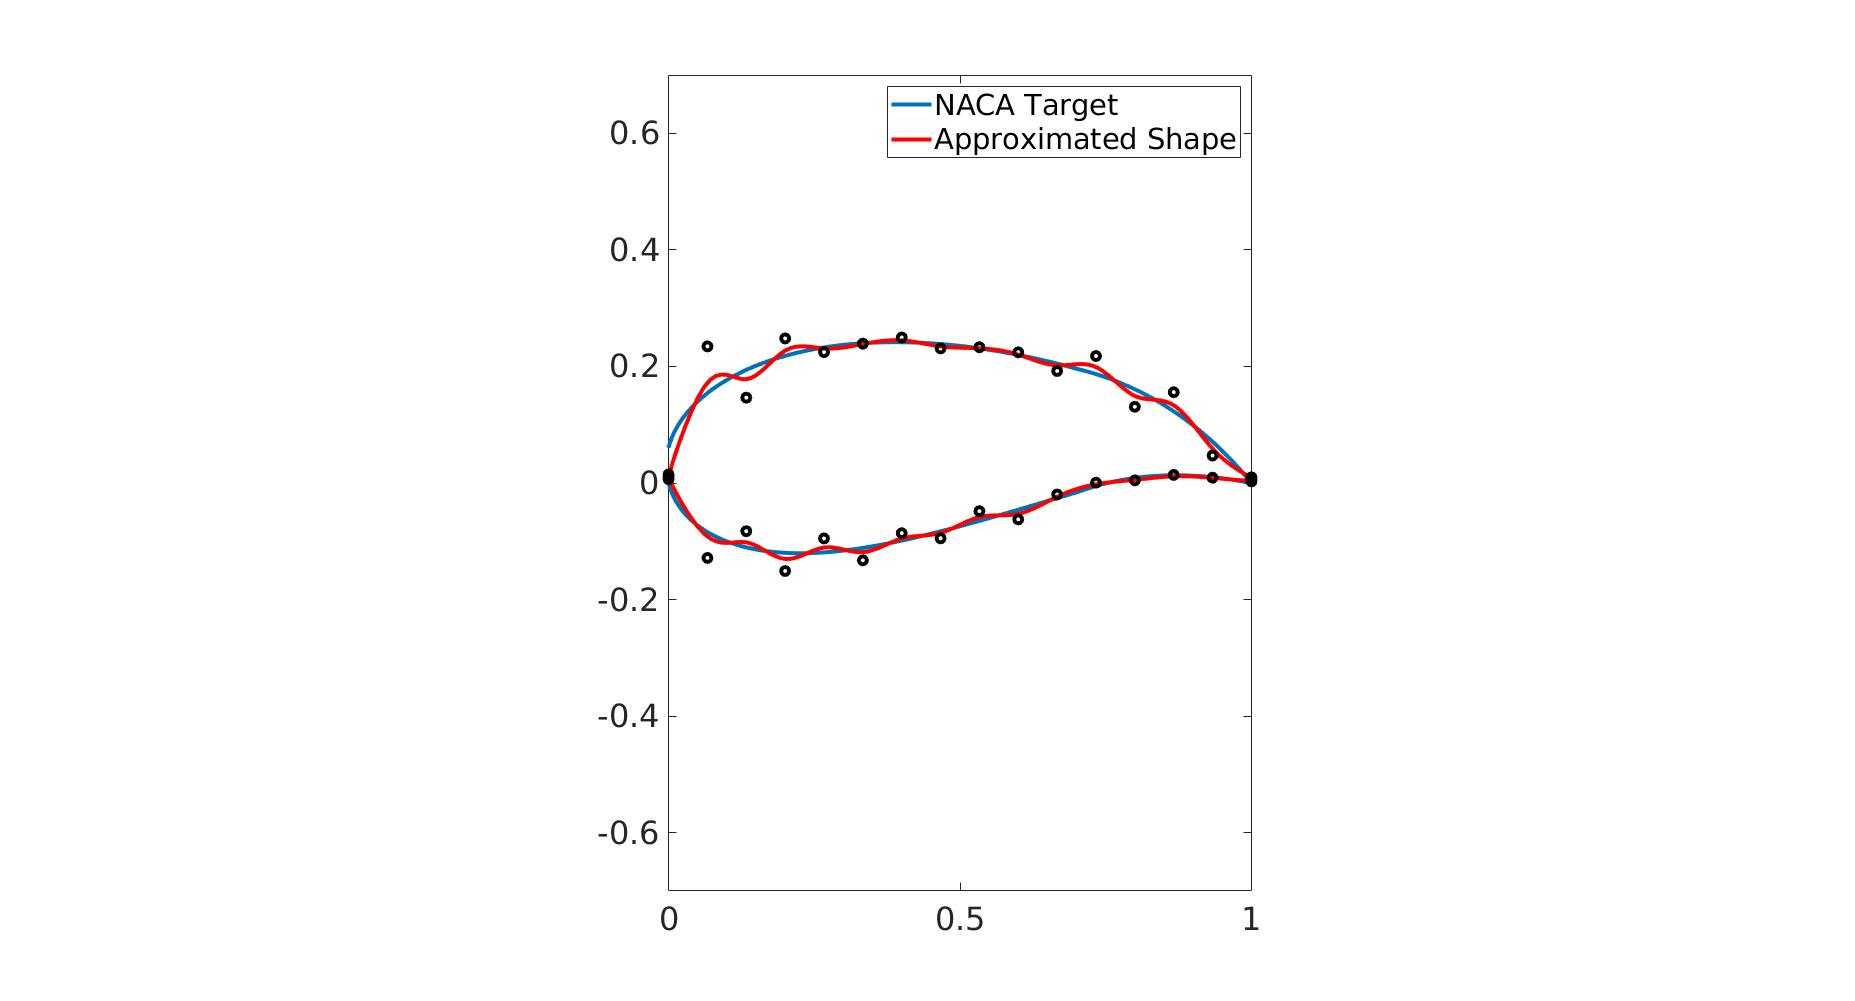
\includegraphics[width=1.0\textwidth]{img/es_foil3_single.jpg}
				\caption{Plot on NACA [9, 7, 3, 5] with ES}
			\end{figure}
			\begin{figure}[H]
				\centering
				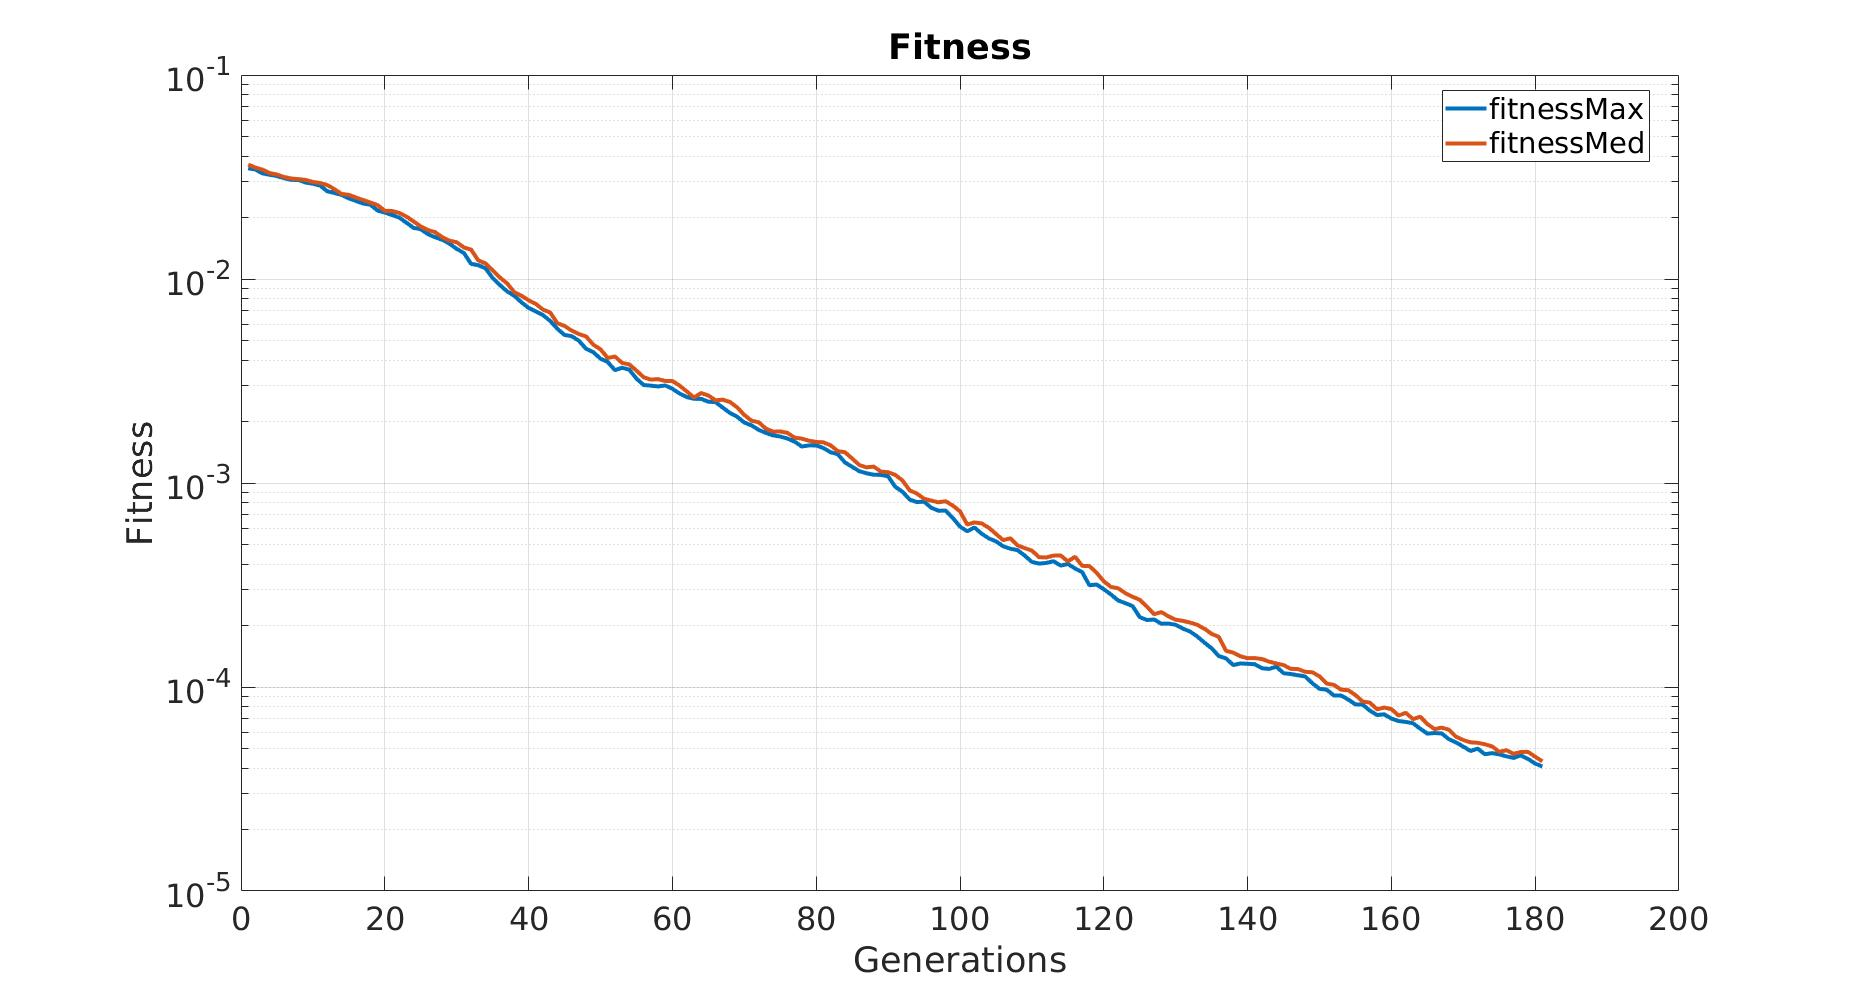
\includegraphics[width=1.0\textwidth]{img/es_fitness_foil3_single.jpg}
				\caption{Fitness plot on NACA [9, 7, 3, 5] with ES}
			\end{figure}
			
			\item Compare to your best GA. Is one significantly better than the other?
			\begin{figure}[H]
				\centering
				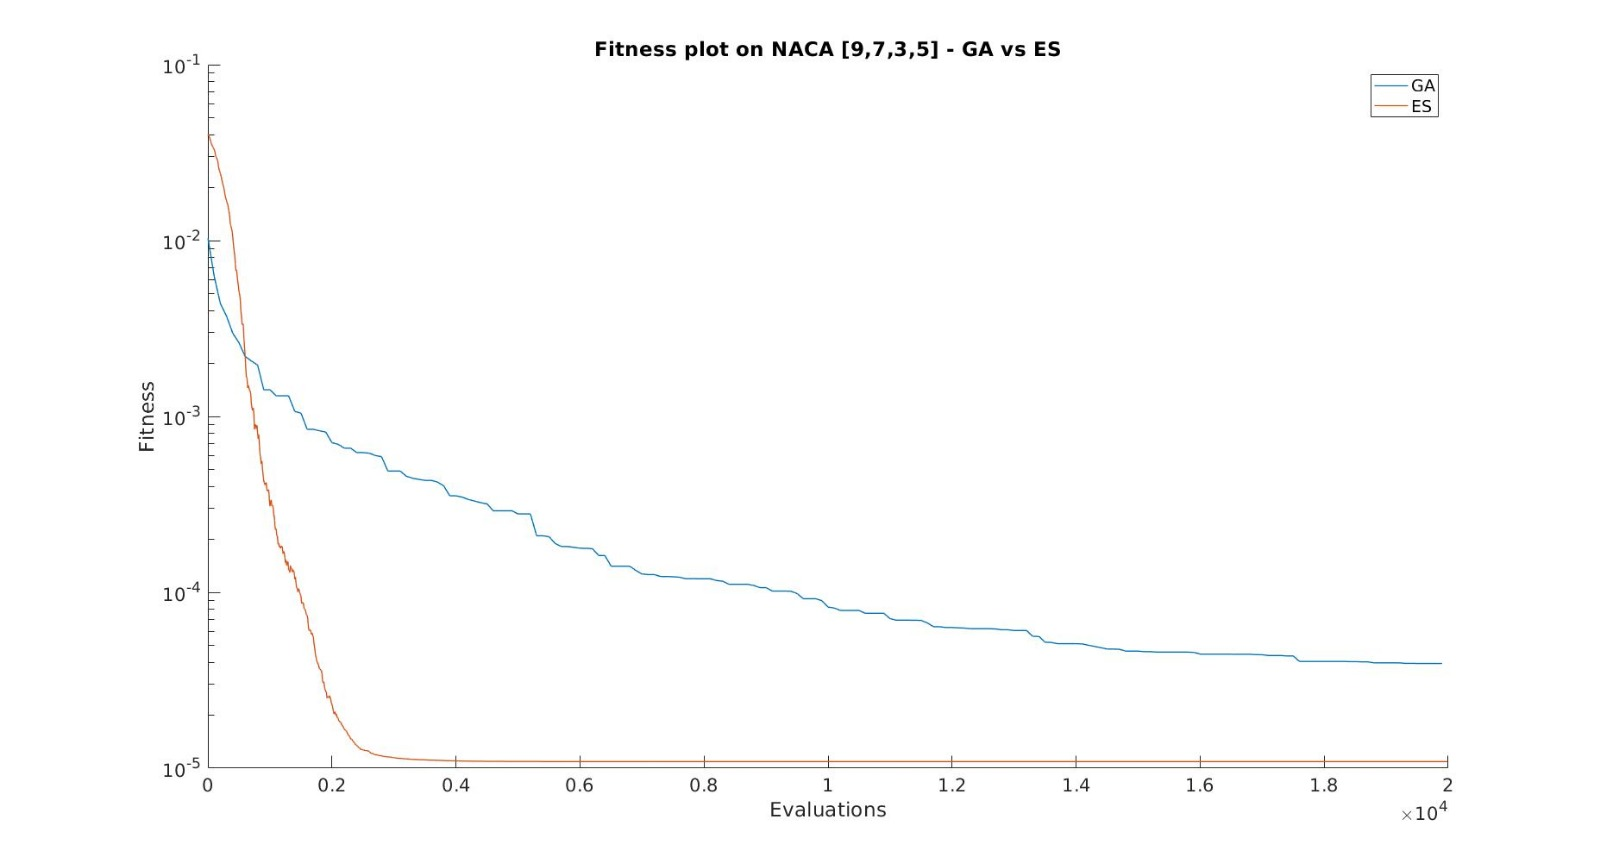
\includegraphics[width=1.0\textwidth]{img/ga_es.jpeg}
			\end{figure}
			\color{blue}
				It is observed that the GA does not manage to converge to the global minima even after 20000 evaluations.
				
				However, the ES manages to converge to the global minima within 2000-2500 evaluations. Thus it can be seen to be significantly better than the GA.			
			\color{black}
			
		\end{itemize}
	\item Now program CMA-ES \underline{without evolution paths}.
	\begin{itemize}
		\item Compare to your ES results. Is a there a significant improvement?	
	\end{itemize}
	\begin{figure}[H]
		\centering
		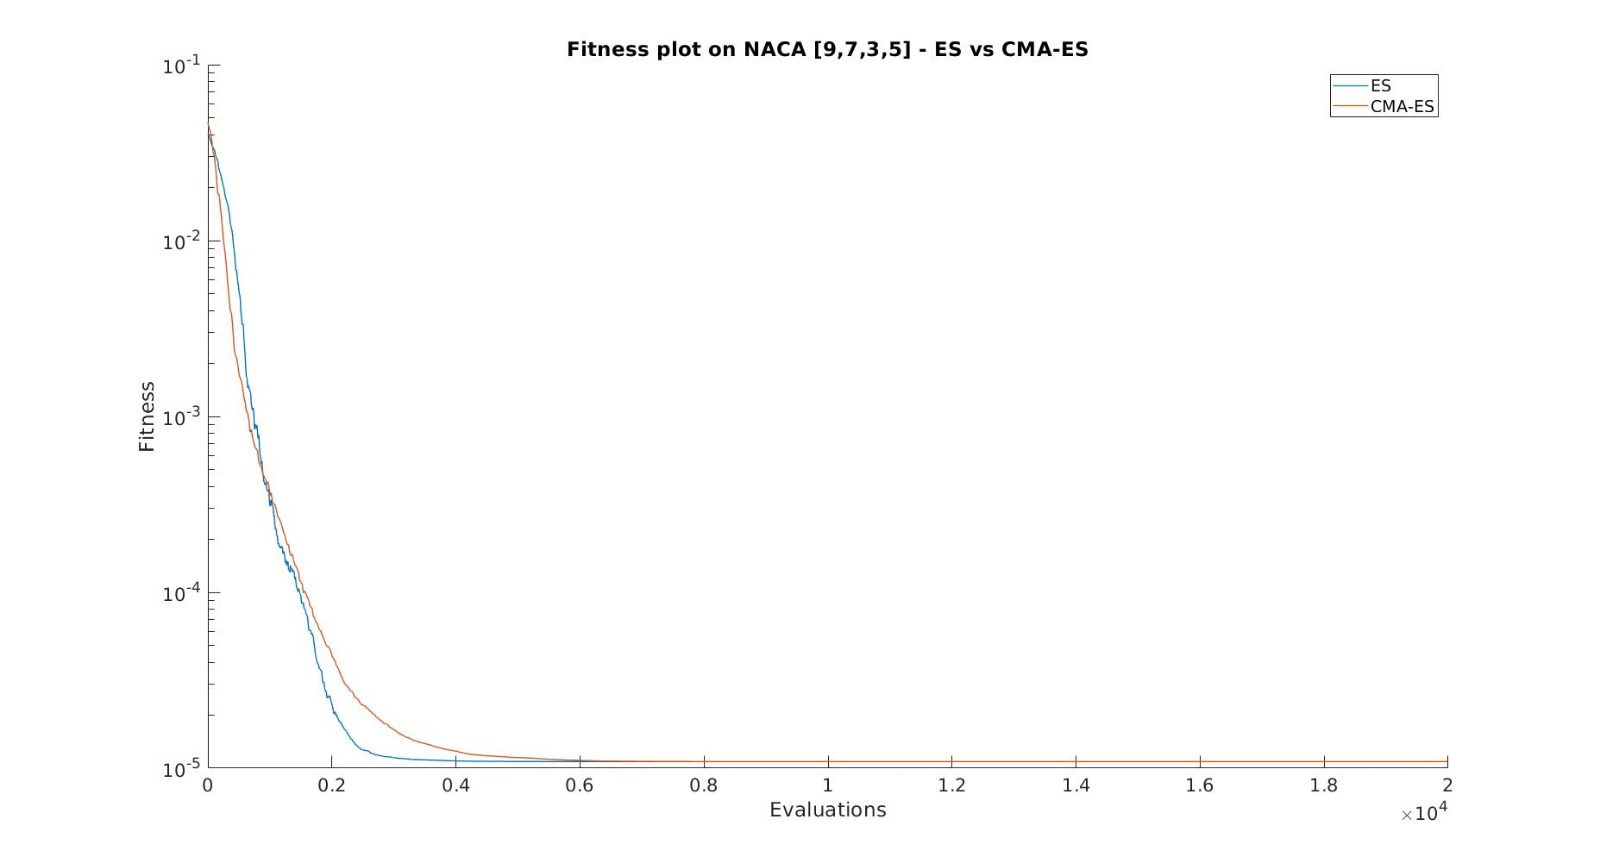
\includegraphics[width=1.0\textwidth]{img/es_cmaes.jpeg}
	\end{figure}
	\color{blue}
	It is observed that both the ES and CMAES manages to converge to the global minima, however, the ES is seen to perform slightly better. This may be attributed to the selection of parameters, including the population size and number of generations.			
	\color{black}
	

	\item \textit{***Extra Credit***} Now program CMA-ES \underline{with evolution paths}.
		\begin{itemize}
		\item Compare to your previous CMA-ES results. Is a there a significant improvement?
		\end{itemize}
		
		\begin{figure}[H]
			\centering
			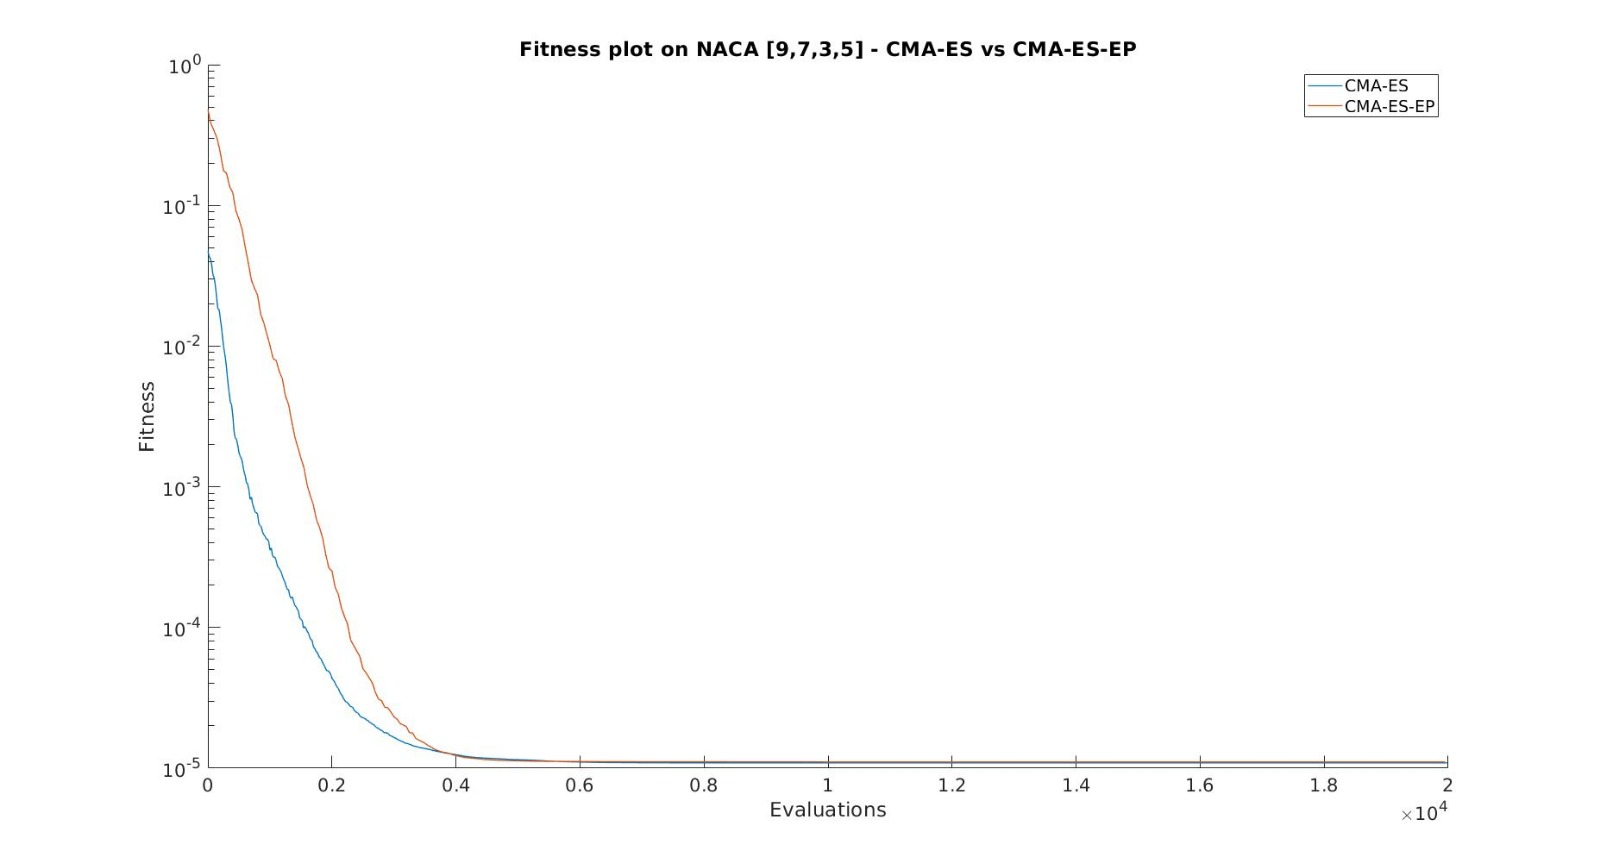
\includegraphics[width=1.0\textwidth]{img/cmaes_cmaesep.jpeg}
		\end{figure}
		\color{blue}
		CMAES-EP is seen to converge slightly faster than the CMAES. This can be attributed to the fact that the path of evolution adapts the way the step sizes are updated, thus leading to faster convergence.
		\color{black}
\end{itemize}

\newpage
\subsection{Comparisons}
Produce one plot which shows the performance of each algorithm. Run each algorthm 20 times on each shape (NACA airfoil shapes: 0012, 5522, 9735), with a budget of 20,000 function evaluations. For each run record the best ever found individual at each evaluation. For each algorithm plot the median fitness of this best ever individual. This may take some time, write a script to run and collect this data. The following should be on this plot (leaving out any algorithms you chose not to implement):
\begin{enumerate}
	\item Binary GA
	\item Real-Valued GA
	\item ES
	\item CMA-ES (without evolution paths)
	\item CMA-ES (with evolution paths)
\end{enumerate}

\begin{figure}[H]
	\centering
	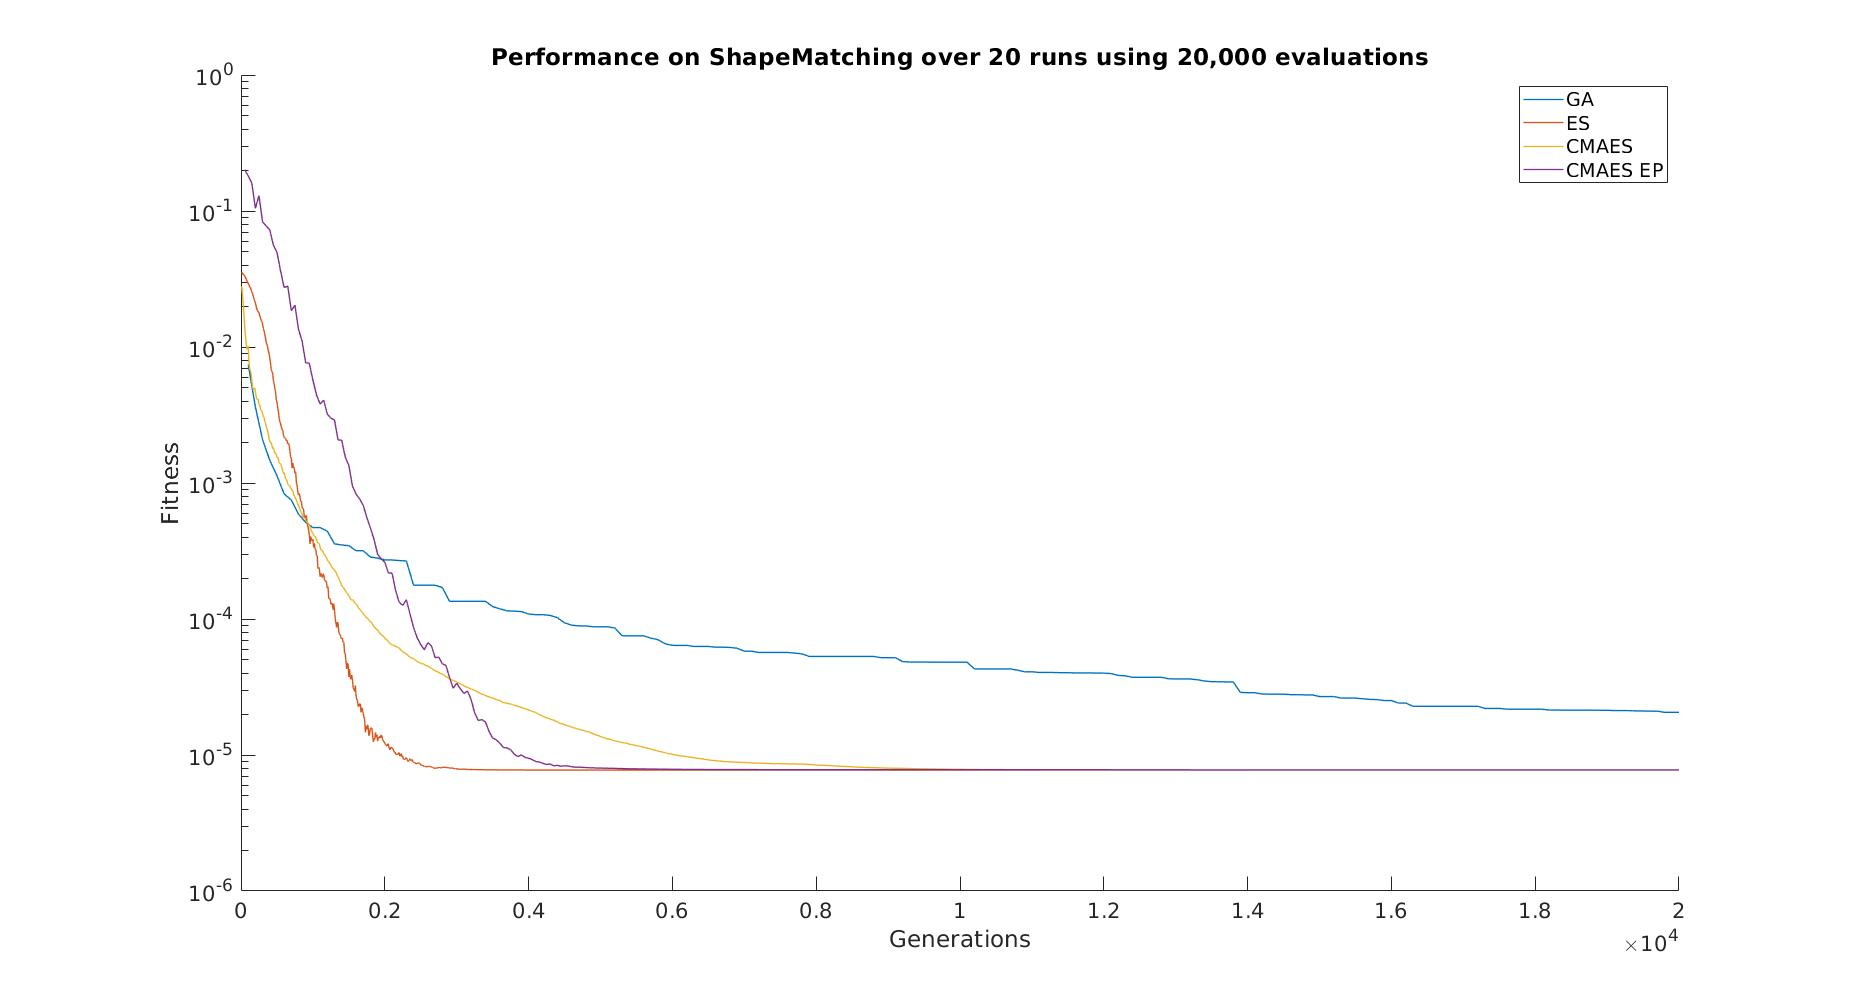
\includegraphics[width=1.0\textwidth]{img/20_runs_2000_all.jpg}
	\caption{Best values across all air foils over 20 runs with 20,000 evaluations each for the GA, ES, CMAES and CMAES EP for the shape matching problem.}
\end{figure}






\end{document}










